\documentclass[11pt, a4paper]{article}
\usepackage[utf8]{inputenc}
\usepackage[margin=.7in]{geometry}
\usepackage{listings}
\usepackage{setspace}
\usepackage{xcolor}
\usepackage{titlesec}
\usepackage{enumitem}
\usepackage{amssymb}
\usepackage{amsmath}
\usepackage{bm}
\usepackage{multicol}
\usepackage{graphicx}
\graphicspath{{./Figures/}}
\usepackage{color}
\usepackage{hyperref}
\hypersetup{
	colorlinks=true,
	linkcolor=blue,
	urlcolor=blue,
}
\titleformat*{\section}{\LARGE\bfseries\filcenter}
\titleformat*{\subsection}{\Large\bfseries}
\titleformat*{\subsubsection}{\large\bfseries}
\definecolor{codegreen}{rgb}{0,0.5,0}
\definecolor{codegray}{rgb}{0.5,0.5,0.5}
\definecolor{codered}{rgb}{0.78,0,0}
\definecolor{codepurple}{rgb}{0.58,0,0.68}
\definecolor{backcolour}{rgb}{0.95,0.95,0.92}
\lstdefinestyle{mystyle}{
    backgroundcolor=\color{backcolour},   
    commentstyle=\color{gray},
    keywordstyle=\color{codegreen},
    numberstyle=\tiny\color{codegray},
    stringstyle=\color{codered},
    basicstyle=\ttfamily\footnotesize,
    breakatwhitespace=false,         
    breaklines=true,                 
    captionpos=b,                    
    keepspaces=true,                 
    numbers=left,                    
    numbersep=5pt,                  
    showspaces=false,                
    showstringspaces=false,
    showtabs=false,                  
    tabsize=2,
    morekeywords = {as},
    keywordstyle = \color{codegreen}
}
\lstset{style=mystyle}

\begin{document}
	\begin{titlepage}
		\begin{center} \Huge \textbf{Data Science} \end{center}
		\tableofcontents
		\newpage
	\end{titlepage}
%%%% PAGE 1 %%%%
	\begin{spacing}{1.1}
	\section{Introduction to SQL}
	\subsection{Relational Database Management System}
	A \textbf{database} is a set of data stored in a computer. This data is usually structured in a way that makes the data easily accessible. A \textbf{relational database} is a type of database. It uses a structure that allows us to identify and access data in \textit{relation} to another piece of data in the database. Often, data in a relational database is organized into tables with records (rows) and columns. \vspace*{1mm}\\
	A \textbf{relational database management system (RDBMS)} is a program that allows you to create, update, and administer a relational database. Most use SQL language to access the database. However, SQL syntax can differ based on  which RDBMS you are using. \\
	
	\subsection{Data Manipulation in SQL}
	- A statement always ends in a semicolon \textbf{;} \vspace*{1mm}\\
	Components of a statement: \\
	1) Clause -  perform specific task is SQL, written in capital letters (known as commands) \\
	2) Table name - written in lowercase letters, name of table to apply command to \\
	3) Parameters - list of columns, data types, or values that are passed to a clause as an argument\\~\\
	The \textbf{CREATE} statement allows use to create a new table in the database 
	\begin{lstlisting}[language=SQL]
	CREATE TABLE table_name (
		column1 datatype,
		column2 datatype,
		column3 datatype
	);	\end{lstlisting} \vspace*{1mm}
	The \textbf{INSERT} and \textbf{VALUES} statements allows us to add new records (rows) to a table
	\begin{lstlisting}[language=SQL]
	-- Insert into columns in order:
	INSERT INTO table_name
	VALUES (value1, value2);
	
	-- Insert into columns by name:
	INSERT INTO table_name (column1, column2)
	VALUES (value1, value2);	\end{lstlisting} \vspace*{1mm}
	The \textbf{SELECT} statements will fetch data from a database (query data from database)
	\begin{lstlisting}[language=SQL]
	SELECT column_name FROM table_name;
	SELECT * FROM tabe_name; -- all columns from table \end{lstlisting} \vspace*{1mm}
	The \textbf{ALTER TABLE} adds a new column(s) to the table (will be initialized to NULL ($\emptyset$))
	\begin{lstlisting}[language=SQL]
	ALTER TABLE table_name
	ADD column_name datatype; \end{lstlisting} \vspace*{1mm}
	The \textbf{UPDATE} statement allows use to edit existing records
	\begin{lstlisting}[language=SQL]
	UPDATE table_name
	SET column1 = value1, column2 = value2
	WHERE some_column = some_value; \end{lstlisting} \vspace*{1mm}
	The \textbf{DELETE FROM} statement deletes one or more rows from a table
	\begin{lstlisting}[language=SQL]
	DELETE FROM table_name
	WHERE some_column = some_value; \end{lstlisting} \newpage
%%%% PAGE 2 %%%%
	\noindent \textbf{Constraints} add information about how a column can be used are invoked after specifying the data type for a column. They can be used to tell the database to reject inserted data that does not adhere to a certain restriction. \\
	\hspace*{3mm} - PRIMARY KEY columns uniquely identify a row, only one per table \\
	\hspace*{3mm} - UNIQUE columns have different value for every row, can be multiple per table \\
	\hspace*{3mm} - NOT NULL columns must have a value \\
	\hspace*{3mm} - DEFAULT columns will pass an assumed value if non specified
	\begin{lstlisting}[language=SQL]
	CREATE TABLE student (
		id INTEGER PRIMARY KEY, -- Can't add another row called ID or any of the values
		name TEXT UNIQUE, -- Can't add same value in name row
		grade INTEGER NOT NULL, -- Can't leave value NULL when adding new grade
		age INTEGER DEFAULT 10 -- Passes given parameter if non given
	); \end{lstlisting} \vspace*{5mm}
	
	\subsection{Writing Queries}
	\textbf{Queries} allow us to communicate with the database by asking questions and having the result set return data relevant to the question. One of the core purposes of the SQL language is to retrieve information stored in a database. \\~\\
	The \textbf{SELECT} statement is used to query data from a database, with \textbf{*} meaning all columns 
	\begin{lstlisting}[language=SQL]
	SELECT column1, column2 
	FROM table_name; \end{lstlisting} \vspace*{1mm}
	The \textbf{AS} keyword lets you rename a column or table using an specified alias. However, this doesn't rename the column in the table, only the results outputted
	\begin{lstlisting}[language=SQL]
	SELECT column_name AS 'alias'
	FROM table_name; \end{lstlisting} \vspace*{1mm}
	The \textbf{DISTINCT} keyword allows us to return only unique values in the output, filtering all duplicates
	\begin{lstlisting}[language=SQL]
	SELECT DISTINCT column_name 
	FROM table_name; \end{lstlisting} \vspace*{1mm}
	The \textbf{WHERE} clause lets us restrict our query results where a condition is true ($=,!=,<,>,<=,>=$)
	\begin{lstlisting}[language=SQL]
	SELECT column_name 
	FROM table_name 
	WHERE condition; \end{lstlisting} \vspace*{1mm}
	The \textbf{LIKE} is a special operator used with WHERE to search for a specific pattern in a column \\
	\hspace*{3mm} - The \_ wildcard means substitute any character\\
	\hspace*{3mm} - The \% wildcard means matching zero or more missing letters in the pattern (not case sensitive)
	\begin{lstlisting}[language=SQL]
	SELECT * 
	FROM movies
	WHERE name LIKE 'Se_en'; -- The _ means any character (return 'Seven' and 'Se7en')
	-- WHERE name LIKE 'A%' matches all movies beginning with letter A
	-- WHERE name LIKE '%a' matches all movies end with letter a
	-- WHERE name LIKE '%man%' matches all movies containing 'man' \end{lstlisting} \vspace*{1mm}
	We can test for NULL values with operates \textbf{IS NULL} and \textbf{IS NOT NULL} (can't use = or !=)
	\begin{lstlisting}[language=SQL]
	SELECT column_name
	FROM table_name 
	WHERE column_name IS NULL; -- or IS NOT NULL \end{lstlisting} \vspace*{1mm}
%%%% PAGE 3 %%%%
	The \textbf{BETWEEN} operator is used with WHERE to filter results within a certain range \\
	\hspace*{3mm} - Number ranges include the final value (ex: 1970 AND 1979 includes 1979) \\
	\hspace*{3mm} - Text ranges do not include final value (ex: `A' AND `D' stops before D)
	\begin{lstlisting}[language=SQL]
	SELECT *
	FROM movies
	WHERE year BETWEEN 1990 AND 1999; -- includes 1999
	-- WHERE name BETWEEN 'A' AND 'J'; up to, but not including, J \end{lstlisting} \vspace*{1mm}
	The \textbf{AND} or \textbf{OR} operators to combine multiple conditions in a WHERE clause
	\begin{lstlisting}[language=SQL]
	SELECT * 
	FROM movies
	WHERE year BETWEEN 1990 AND 1999
		AND genre = 'romance'; -- both conditions must be true 
	
	SELECT *
	FROM movies
	WHERE year > 2014 OR genre = 'action'; -- either condition is true \end{lstlisting}  \vspace*{1mm}
	\noindent The \textbf{ORDER BY} lets ys sort results (alphabetic or numeric). We can pass the given keywords: \\
	\hspace*{3mm} - DESC to sort results descending (high-low or Z-A) \\
	\hspace*{3mm} - ASC to sort results ascending (low-high or A-Z) \\
	NOTE: If a WHERE clause is present, the ORDER BY goes after
	\begin{lstlisting}[language=SQL]
	SELECT column_name
	FROM table_name
	ORDER BY column_name DESC; -- can also be ASC (ASC is same as blank) \end{lstlisting} \vspace*{1mm}
	The \textbf{LIMIT} clause lets you specify the max number of rows the result set will have (at end of query)
	\begin{lstlisting}[language=SQL]
	SELECT column_name
	FROM table_name
	LIMIT num_value; -- replace num_value with an integer \end{lstlisting} \vspace*{1mm}
	The \textbf{CASE} statement allows us to create different outputs (SQL's if-then logic). Each WHEN tests a condition and if true, executes the THEN parameter. ELSE parameter is executed if all WHEN tests are false. Always finish CASE statement with END.
	\begin{lstlisting}[language=SQL]
	SELECT name, -- given column name
		CASE
			WHEN genre = 'romance' THEN 'Chill' -- If romance genre then label chill
			WHEN genre = 'comedy' THEN 'Chill' -- if comedy then label chill
			ELSE 'Intense' -- if both above false, then label intense
		END AS 'Mood' -- label column with all results
	FROM movies; -- table to read from \end{lstlisting} \vspace*{5mm}
		
	\subsection{Aggregate Functions}
	We will know learn about \textbf{aggregates} which are calculations performed on multiple rows of a table. \\~\\
	The \textbf{COUNT()} function returns the total number of rows that match the specified criteria (excludes $\emptyset$)
	\begin{lstlisting}[language=SQL]
	SELECT COUNT(column_name) -- can be *
	FROM table_name
	WHERE condition; -- this line is optional \end{lstlisting} \newpage
%%%% PAGE 4 %%%%
	\noindent The \textbf{SUM()} function takes a column name as an argument and returns sum of all values in column.
	\begin{lstlisting}[language=SQL]
	SELECT SUM(column_name)
	FROM table_name; \end{lstlisting} \vspace*{1mm}
	The \textbf{MAX()} and \textbf{MIN()} functions return the highest and lowest values in a column, respectively.
	\begin{lstlisting}[language=SQL]
	SELECT MAX(column_name) -- can also be MIN(column_name)
	FROM table_name; \end{lstlisting} \vspace*{1mm}
	The \textbf{AVG()} function to quickly calculate the average value of a particular column
	\begin{lstlisting}[language=SQL]
	SELECT AVG(column_name)
	FROM table_name; \end{lstlisting} \vspace*{1mm}
	The \textbf{ROUND()} function takes two parameter, a column name and an integer, and rounds the result
	\begin{lstlisting}[language=SQL]
	SELECT ROUND(column_name, integer)
	FROM table_name; \end{lstlisting} \vspace*{1mm}
	The \textbf{GROUP BY} function arranges identical data into groups (NOTE: comes after FROM or WHERE, but before ORDER BY or LIMIT). We can also use GROUP BY on columns by using integers instead of strings (1 = first column select, 2 = second column selected, ...)
	\begin{lstlisting}[language=SQL]
	SELECT price, COUNT(*) -- shows price and count all rows
	FROM fake_apps
	WHERE downloads > 20000 -- where over 20000 downloads
	GROUP BY price; -- sort results by price 
	
	SELECT category, price, AVG(downloads)
	FROM fake_apps
	GROUP BY 1, 2; -- groups by category and price \end{lstlisting} \vspace*{1mm}
	The \textbf{HAVING} function filters groups for a query built with aggregate properties (similar to WHERE)\\
	NOTE: HAVING always comes after GROUP BY but before ORDER BY and LIMIT
	\begin{lstlisting}[language=SQL]
	SELECT price, ROUND(AVG(downloads)), COUNT(*)
	FROM fake_apps
	GROUP BY price -- group by price
	HAVING COUNT(name) > 10; -- filter groups where they must have 10+ apps \end{lstlisting} \vspace*{1mm}
	The \textbf{strftime()} function takes two parameters, the format a column name \\
	\hspace*{3mm} - Formats: Click \href{https://www.sqlite.org/lang_datefunc.html}{this} link to see all the format options
	\begin{lstlisting}[language=SQL]
	SELECT timestamp,
	strftime('%H', timestamp) -- returns the hour of our timestamp column
	FROM hacker_news
	GROUP BY 1
	LIMIT 20; \end{lstlisting} \vspace*{1mm}
	FROM `THE MET' PROJECT
	\begin{lstlisting}[language=SQL]
	SELECT CASE
		WHEN medium LIKE '%gold%'   THEN 'Gold' -- any art piece with gold in name
		WHEN medium LIKE '%silver%' THEN 'Silver' -- any art piece with silver in name
		ELSE NULL -- all other art pieces are NULL
	 END AS 'Bling', -- rename results column as Bling
	 COUNT(*) -- part of select statement to count all rows
	FROM met
	WHERE Bling IS NOT NULL -- discard all non gold/silver pieces
	GROUP BY 1 -- group by CASE column
	ORDER BY 2 DESC; -- order by number of items (COUNT) \end{lstlisting} \newpage
%%%% PAGE 5 %%%%
	\subsection{Multiple Tables}
	In order to efficiently store data, we often spread related information across multiple tables. \vspace*{2mm}\\
	The \textbf{JOIN} function lets us combine tables easily. This simple JOIN is called an \textit{inner join}, and will only include rows that have matching values, but will omit any rows not matching our ON condition.
	\begin{lstlisting}[language=SQL]
	SELECT * -- all columns
	FROM orders -- from orders table
	JOIN subscriptions -- joined with subscriptions table
		ON orders.subscription_id = subscriptions.subscription_id -- match these columns
	WHERE subscriptions.description = 'Fashion Magazine'; -- only for this description \end{lstlisting} \vspace*{1mm}
	The \textbf{LEFT JOIN} allows us to combine two tables and keep the unmatched rows we would lose in the inner join (keeps all values from the left table in the FROM statement and fills in missing values in the right table with NULL values)
	\begin{lstlisting}[language=SQL]
	SELECT * -- select all columns
	FROM newspaper -- keep all rows from newspaper table
	LEFT JOIN online -- join with online table
		ON newspaper.id = online.id -- match these columns
	WHERE online.id IS NULL; -- see who subscribes to newspaper but not online \end{lstlisting} \vspace*{1mm}
	A \textbf{Primary Key} is a column that uniquely identifies each row of a table. They have a few requirements: \\
	\hspace*{3mm} - None of the values can be NULL \\
	\hspace*{3mm} - Each value is unique (no 2 rows with same value) \\
	\hspace*{3mm} - A table can only have one primary key column \\
	Now, when a primary key for one table appears in a different table, it is a \textbf{Foreign Key}. This is important because the most common types of joins will be joining a foreign key from one table to the primary key from another table.
	\begin{lstlisting}[language=SQL]
	SELECT * 
	FROM classes -- primary key = id
	JOIN students -- primary key = id, foreign_key = class id 
		ON classes.id = students.class_id; -- join primary key with foreign key \end{lstlisting} \vspace*{1mm}
	The \textbf{CROSS JOIN} lets all combine all rows of one table with all rows of another table (think of as finding all possible combinations of the two tables).
	\begin{lstlisting}[language=SQL]
	SELECT month, COUNT(*) AS 'subscribers' -- columns to display
	FROM newspaper -- table 1
	CROSS JOIN months -- table 2
	WHERE start_month <= month AND end_month >= month -- where user was subscribed
	GROUP BY month; -- group together results by month \end{lstlisting}\vspace*{1mm}
	The \textbf{UNION} operator lets us stack data sets on top of one another, given that thy have the same number of columns and the columns have the same data types.
	\begin{lstlisting}[language=SQL]
	SELECT *
	FROM table_name1
	UNION
	SELECT * 
	FROM table_name2; -- will put table_name2 below table_name1 \end{lstlisting} \newpage
%%%% PAGE 6 %%%%
	\noindent The \textbf{WITH} clause allows us to perform a separate query and store it in a temporary table that we can reference any columns from. We can then join this temporary table with another table
	\begin{lstlisting}[language=SQL]
	WITH previous_query AS ( -- create a temp table
		SELECT customer_id, COUNT(subscription_id) AS 'subscriptions' -- select columns
		FROM orders -- table
		GROUP BY customer_id -- grouped by customer id
	) -- end of our temp table query
	SELECT customers.customer_name, previous_query.subscriptions -- new col., temp col.
	from previous_query -- from temp table
	JOIN customers -- inner join with cutomers table
		ON previous_query.customer_id = customers.customer_id; -- if parameters met \end{lstlisting} \vspace*{4mm}
		
	\subsection{Usage Funnels}
	A \textbf{funnel} is a marketing model which illustrates the theoretical customer journey towards the purchase of a product or service. Oftentimes, we want to track how many users complete a series of steps and know which steps have the most number of users giving up. \\~\\
	We can \textbf{build a funnel from a single table}. Lets count the distinct users who answered each question.
	\begin{lstlisting}[language=SQL]
	SELECT question_text, COUNT(DISTINCT user_id)
	FROM survey_responses
	GROUP BY 1; \end{lstlisting}\vspace*{1mm}
	We can \textbf{compare funnels for A/B tests}. Half of the users view the original control version and half view the new variant version, lets count the control and variant clicks for each modal step
	\begin{lstlisting}[language=SQL]
	SELECT modal_text, 
		COUNT(DISTINCT CASE
			WHEN ab_group = 'control' THEN user_id
			END) AS 'control_clicks', -- creat column for control clicks
		COUNT(DISTINCT CASE
			WHEN ab_group = 'variant' THEN user_id
			END) AS 'variant_clicks' -- create column for version clicks
	FROM onboarding_modals
	GROUP BY 1
	ORDER BY 1; \end{lstlisting}\vspace*{1mm}
	We can also \textbf{build a funnel from multiple tables}. In the end, we want to see if the conversion rate from checkout to purchase changes as we get closer to Christmas.
	\begin{lstlisting}[language=SQL]
	WITH funnels AS (
		SELECT DISTINCT b.browse_date, -- distinct browse dates
			b.user_id, -- get all user id's
			c.user_id IS NOT NULL AS 'is_checkout', -- 1 if in checkout, 0 if not
			p.user_id IS NOT NULL AS 'is_purchase' -- 1 if purchased, 0 if not
		FROM browse AS 'b' -- rename table browse as b
		LEFT JOIN checkout AS 'c' -- join c with b
			ON c.user_id = b.user_id -- match c user id to b user id
		LEFT JOIN purchase AS 'p' -- join p with bc table
			ON p.user_id = c.user_id) -- match p user id to bc table user id
	SELECT browse_date, COUNT(*) AS 'num_browse', -- browse dates, users in browse stage
		SUM(is_checkout) AS 'num_checkout', -- total number in checkout stage
		SUM(is_purchase) AS 'num_purchase', -- total numberin  purchased stage
		1.0 * SUM(is_checkout) / COUNT(user_id) AS 'browse_to_checkout', -- b:c ratio
		1.0 * SUM(is_purchase) / SUM(is_checkout) AS 'checkout_to_purchase' -- c:p ratio
	FROM funnels -- from temp table
	GROUP BY 1 -- group by browse date
	ORDER BY 1; -- order by browse date (ASC) \end{lstlisting} \newpage
%%%% PAGE 7 %%%%
	\noindent USAGE FUNNELS WITH WARBY PARKER PROJECT 
	\begin{lstlisting}[language=SQL]
	WITH temp_results AS ( -- create temp table
		SELECT DISTINCT q.user_id, 
			ht.user_id IS NOT NULL AS 'is_home_try_on', -- 0 if no glasses, 1 if has glasses
			ht.number_of_pairs, -- 3 pairs, 5 pairs (A/B testing)
			p.user_id IS NOT NULL as 'is_purchase' -- 0 if no purchase, 1 if purchase
		FROM quiz q -- quiz table referenced as q
		LEFT JOIN home_try_on ht 
			ON q.user_id = ht.user_id -- where user id's match
		LEFT JOIN purchase p
			ON q.user_id = p.user_id -- where user id's match
		WHERE ht.number_of_pairs IS NOT NULL ) -- customer has either A/B test
	SELECT number_of_pairs AS 'Try On Pairs', -- 3 or 4 pairs 
		COUNT(*) AS 'Customers', -- total for customers
		SUM(is_purchase) AS 'Purchased Product', -- if customer bought product
		1.0 * SUM(is_purchase) / COUNT(*) AS 'Purchase Rate' -- rate of purchase
	FROM temp_results -- from temp table above
	GROUP BY 1 -- group by pair type
	ORDER BY 4 DESC; -- order by purchase rate 
	-- We see that 5 pairs purchase rate = 79%, 3 pairs purchase rate = 53% \end{lstlisting}\vspace*{4mm}
	
	\subsection{User Churn}
	\textbf{Churn rate} is the percent of subscribers that have canceled within a certain period, usually a month. For a user base to grow, the churn rate must be less than the new subscriber rate for the same period and is calculated by $\frac{cancellations}{total\;subscribers}$.\\~\\
	We can calculate churn for a month from a single table 
	\begin{lstlisting}[language=SQL]
	SELECT 1.0 * (
		SELECT COUNT(*)
		FROM subscriptions
		WHERE subscription_start < '2017-01-01' 
		AND (subscription_end BETWEEN '2017-01-01' AND '2017-01-31')
	 ) / (
		SELECT COUNT(*)
		FROM subscriptions
		WHERE subscription_start < '2017-01-01'
		AND ((subscription_end >= '2017-01-01') 
			OR (subscription_end IS NULL))
	) AS results; \end{lstlisting}\newpage
	
	
	\section{Introduction to Python}
	\subsection{Lists}
	We can use \textbf{zip()} to create pairs from multiple lists. However, it returns the location in memory and must be converted back to a \textbf{list()} in order to print it.\\ 
	We can add a single element to a list using \textbf{.append()}, which will place at the end of the list. \\
	We can add multiple lists together by using $\bm{+}$ to concatenate them.
	\begin{lstlisting}[language=Python]
	last_semester_gradebook = [("politics", 80), ("latin", 96), ("dance", 97), 
	                           ("architecture", 65)]
	
	subjects = ["physics", "calculus", "poetry", "history"]
	grades = [98, 97, 85, 88]
	subjects.append("computer science")
	grades.append(100)
	gradebook = list(zip(subjects,grades)) # combine and cast as a list
	gradebook.append(("visual arts", 93)) # append a tuple
	print(gradebook)
	
	full_gradebook = gradebook + last_semester_gradebook
	print(full_gradebook) \end{lstlisting}\vspace*{1mm}
	We can create an array of integers for a given size by \textbf{range()}, which generates starting at a point (0 by default) to the (input value - 1). However, you must convert it to a list since it returns on object.
	\begin{lstlisting}[language=Python]
	my_list = range(9) # values 0 to 8
	my_list_2 = range(5, 15, 3) # start at 5, end at 14, increment by 3
	print(list(my_list_2)) # [5, 8, 11, 14] \end{lstlisting}\vspace*{1mm}
	We can select a section of a list by using syntax array[start:stop], called \textbf{slicing}. 
	\begin{lstlisting}[language=Python]
	suitcase = ['shirt', 'shirt', 'pants', 'pants', 'pajamas', 'books']
	start = suitcase[:3] # same as suitcase[0:3]
	end = suitcase[-2:] # gets last 2 elements of suitcase \end{lstlisting}\vspace*{1mm}
	We can count how many times an element appears in a list with \textbf{.count()}
	\begin{lstlisting}[language=Python]
	votes = ['Jake', 'Jake', 'Laurie', 'Laurie', 'Laurie', 'Jake']
	jake_votes = votes.count('Jake')
	print(jake_votes) \end{lstlisting}\vspace*{1mm}
	We can sort a list alphabetically or numerically with \textbf{.sort()} - only alters a list, doesn't return a value \\
	We can use \textbf{sorted()} to also sort a list, but it will not affect the original list (returns sorted copy)
	\begin{lstlisting}[language=Python]
	games = ['Portal', 'Minecraft', 'Pacman', 'Tetris', 'The Sims', 'Pokemon']
	
	games_sorted = sorted(games)
	print(games) # in same order as above
	print(games_sorted) # new list of sorted games
	
	games.sort()
	print(games) # now the games list is also sorted \end{lstlisting}\vspace*{1mm}
	\textbf{Tuples} are immutable (can't change any values after creating) and are denoted with ( ) \\
	We use tuples to store data that belongs together and don't need order or size to change
	\begin{lstlisting}[language=Python]
	my_info = ('Derek', 22, 'Student')
	name, age, occupation = my_info # will assign each value to a varaible
	
	one_element_tuple = (4,) # NOTE: we need the , after 4 otherwise it wont be a tuple
	one_element_tuple_2 = (4) # same as one_element_tuple_2 = 4	 \end{lstlisting} \newpage
%%%% PAGE 9 %%%%
	
	\subsection{Loops}
	We can use \textbf{for} loops to iterate through each item in a list, with the following general formula \\
	\hspace*{3mm} - We can use range() to execute a for loop from start (0 by default) to stop (n-1) \\
	\hspace*{3mm} - We can use \textit{break} to exit a for loop when a certain value is found \\
	\hspace*{3mm} - We can use \textit{continue} to move to the next index in a list if a condition is found \\
	If we have a list made of multiple lists, we use \textbf{nested} loops to iterate through them
	\begin{lstlisting}[language=Python]
	sales_data = [[12, 17, 22], [2, 10, 3], [5, 12, 13]]
	scoops_sold = 0
	
	for location in sales_data: # for each list in list
		for sales in location: # for each element in inner list
			scoops_sold += sales
	
	print(scoops_sold) \end{lstlisting}\vspace*{1mm}
	We can use \textbf{list comprehension} to efficiently iterate through a list instead of a for loop \\
	We can also use this to alter values in a list and create a new list
	\begin{lstlisting}[language=Python]
	heights = [161, 164, 156, 144, 158, 170, 163, 163, 157] # in cm's
	
	can_ride_coaster = [cm for cm in heights if cm > 161]
	print(can_ride_coaster) # [164, 170, 163, 163] 
	
	celsius = [0, 10, 15, 32, -5, 27, 3] # degrees in C
	
	fahrenheit = [f_temp * (9/5) + 32 for f_temp in celsius] # convert C to F degrees
	print(fahrenheit) # [32.0, 50.0, 59.0, 89.6, 23.0, 80.6, 37.4] \end{lstlisting}\vspace*{4mm}
	
	\subsection{List Comprehension / Lambda Functions}
	We can iterate through lists within lists with the following syntax
	\begin{lstlisting}[language=Python]
	nested_lists = [[4, 8], [15, 16], [23, 42]]
	
	product = [(val1 * val2) for (val1, val2) in nested_lists]
	print(product) # [32, 240, 966]	
	
	greater_than = [ (val1 > val2) for (val1, val2) in nested_lists]
	print(greater_than) # [False, False, False] \end{lstlisting}\vspace*{1mm}
	We can iterate through two lists in one list comprehension by using the zip() function.
	\begin{lstlisting}[language=Python]
	x_values_1 = [2*index for index in range(5)] # [0.0, 2.0, 4.0, 6.0, 8.0] 
	x_values_2 = [2*index + 0.8 for index in range(5)] # [0.8, 2.8, 4.8, 6.8, 8.8] 
	
	x_values_midpoints = [(x1 + x2)/2.0 for (x1, x2) in zip(x_values_1, x_values_2)]
	# [0.4, 2.4, 4.4, 6.4, 8.4]	
	
	names = ["Jon", "Arya", "Ned"]
	ages = [14, 9, 35]
	
	users = ["Name: " + n + ", Age: " + str(a) for (n,a) in zip(names,ages)]
	print(users) # ['Name: Jon, Age: 14', 'Name: Arya, Age: 9', 'Name: Ned, Age: 35'] \end{lstlisting}\newpage
%%%% PAGE 10 %%%%
	\noindent A lambda function is a one-line shorthand for a simple function. It allows us to efficiently run an expression and produce an output for a specific task, such as defining a column in a table, or populating information in a dictionary. It has the following format: \\
	\textit{variableName} = lambda \textit{parameters} : \textit{return value} \vspace*{2mm} \\
	We can also use an if... else... loops within a lambda function with the following format: \\
	(RETURN IF STATEMENT IS TRUE) if (STATEMENT) else (RETURN IF STATEMENT IS FALSE)
	\begin{lstlisting}[language=Python]
	even_or_odd = lambda num : "even" if (num%2 == 0) else "odd"
	
	print even_or_odd(10) # even
	print even_or_odd(5) # odd 
	
	import random as r
	add_random = lambda num : num + r.randint(1,10) # add random int from 1 to 10 to num
	
	print add_random(5)
	print add_random(100) \end{lstlisting}\vspace*{5mm}
	
	\section{Data Analysis with Pandas}
	\subsection{Introduction to Pandas}
	You can pass a \textbf{dictionary} into a DataFrame, where each key is a column name and each value is a list of column values (rows). Note that column lengths must all be the same length or you will get an error.
	\begin{lstlisting}[language=Python]
	import pandas as pd
	
	df1 = pd.DataFrame({
		'Product ID': [1, 2, 3, 4],
		'Product Name' : ['t-shirt', 't-shirt', 'skirt', 'skirt'],
		'Color' : ['blue', 'green', 'red', 'black']
	}) \end{lstlisting}\vspace*{1mm}
	You can also pass a \textbf{list of lists}, where each inner list represents a row of data. You must also add the keyword `columns=' at the end to pass a list of column names.
	\begin{lstlisting}[language=Python]
	df = pd.DataFrame([
		['January', 100, 100, 23, 100],
		['February', 51, 45, 145, 45],
		['March', 81, 96, 65, 96],
		['April', 80, 80, 54, 180],
		['May', 51, 54, 54, 154],
		['June', 112, 109, 79, 129]],
		columns=['month', 'clinic_east', 'clinic_north', 'clinic_south', 'clinic_west']) \end{lstlisting}\vspace*{1mm}
	We can access a \textbf{CSV} (comma separated values) from within pandas. We can get CSV's from online data sets, export from Excel, and export from SQL (assume we read a CSV into a variable df). \\
	\hspace*{4mm} - We can load a CSV file with pd.read\_csv(`filename.csv') \\
	\hspace*{4mm} - We can save data to a CSV with df.to\_csv(`newFilename.csv') \\
	\hspace*{4mm} - The df.head(n) method gives the first n rows of a dataFrame (5 is no n given) \\
	\hspace*{4mm} - The df.info() method gives statistics about each column (data types, etc.) \newpage
%%%% PAGE 11 %%%%
	\noindent We can access \textbf{specific columns} from a DataFrame by using df[`columnName'] or df.columnName (we use the second option of the column has no spaces or special characters). This call will return a Series. \\
	\hspace*{4mm} - We can access \textbf{multiple columns} by passing a list of column names as the parameter. Note that \hspace*{7mm} this will return a DataFrame data type, not a Series.
	\begin{lstlisting}[language=Python]
	# use df from above (list of lists example)
	clinic_north = df.clinic_north # same as df['clinic_north']
	print(type(clinic_north)) # pandas.core.frame.Series
	
	clinic_north_south = df[['clinic_north', 'clinic_south']]
	print(type(clinic_north_south)) # pandas.core.frame.DataFrame \end{lstlisting}\vspace*{1mm}
	We can access \textbf{specific rows} that are \textit{indexed numerically} by using the df.iloc[n] function for any n in our rows. Note that this will also return a Series data type. \\
	\hspace*{4mm} - We can access \textbf{multiple rows} by using splicing on our .iloc[ ] call 
	\begin{lstlisting}[language=Python]
	march = df.iloc[2] # gives us all column values for March row
	april_may_june = df.iloc[3:7] # gives row 3 to 6 and all corresponding column values
	# note that we can also splice from the end using negative numbers \end{lstlisting}\vspace*{1mm}
	We can create \textbf{subsets} of a DataFrame by using logical statements \\
	\hspace*{4mm} - We can combine multiple logical statements with ( ) 
	\hspace*{4mm} - We can use the .isin( ) function to see if a value is in a column
	\begin{lstlisting}[language=Python]
	january = df[df.month == 'January'] # gives all row values if column value is January
	
	march_april = df[(df.month == 'March') | (df.month == 'April')]
	# the above call will gives all row values where month column is March or April
	
	jan_feb_mar = df[df.month.isin(['January', 'February', 'March'])]
	# the above call gives all row values if the .isin parameters are in the month column\end{lstlisting}\vspace*{1mm}
	When we select a subset of a DataFrame using logic, we get non-consecutive indices and is hard to use .iloc[ ] but we can \textbf{change indices} by using .reset\_index( ) to change. \\ 
	\hspace*{4mm} - This function also puts old indices in a new column, to avoid this use keyword drop=True \\
	\hspace*{4mm} - This function will also return a new DataFrame, but to modify our existing use inplace=True
	\begin{lstlisting}[language=Python]
	df2 = df.loc[[1, 3, 5]] # indices are 1, 3, and 5
	df2.reset_index(inplace=True, drop=True) # reset to 0,1,2 and drop old indices column\end{lstlisting}\vspace*{4mm}
	
	\subsection{Modifying DataFrames}
	We can \textbf{add a column} to an existing DataFrame (new information or calculations from data we already have) by giving a list the \textit{same length} as the existing DataFrame. We can do this a few ways.
	\begin{lstlisting}[language=Python]
	# Add a new column to a DataFrame (assume there are 4 rows)
	df['Sold in Bulk?'] = ['Yes', 'Yes', 'No', 'No']
	
	# We can also set an entire column to the same value for every row
	df['Is taxed?'] = 'Yes' # create a new column with 'Yes' in each row
	
	# lets calculate the difference between 2 columns and create a new column from result
	df['Margin'] = df.Price - df['Cost to Manufacture'] 
	#note the difference in calls to the columns due to spaces in column name \end{lstlisting} \newpage
%%%% PAGE 12 %%%%
	\noindent We can use the \textbf{apply()} function to apply a function to every value in a particular column
	\begin{lstlisting}[language=Python]
	from string import lower
	
	df['Lowercase Name'] = df.Name.apply(lower)
	# create a new column from the Name column and apply the lowercase function to it \end{lstlisting}\vspace*{1mm}
	We can use the \textbf{lambda} function to perform complex operations on columns or rows. \\
	\hspace*{4mm} - To operate on \textbf{multiple columns} at once we don't specify a particular column and add the argument \hspace*{7mm} axis=1 (making the input to our lambda an entire row and not a column). \\
	\hspace*{4mm} - To access a particular value of a row, use row.column\_name or row[`column\_name']
	\begin{lstlisting}[language=Python]
	# Apply lambda to a column
	df = pd.read_csv('employees.csv')
	get_last_name = lambda x : x.split(' ')[-1]  # split on space & return end of string
	
	df['last_name'] = df.name.apply(get_last_name)
	
	# Apply plambda to a row (calculate hourly wage)
	total_earned = lambda row: (row.hourly_wage * 40) + ((row.hourly_wage * 1.5) * \ 
	(row.hours_worked - 40)) if row.hours_worked > 40 \
	else row.hourly_wage * row.hours_worked
	
	df['total_earned'] = df.apply(total_earned, axis = 1) \end{lstlisting}\vspace*{1mm}
	We can \textbf{rename} columns so that they are easier to access or read. We can do this a few ways. \\
	\hspace*{4mm} - To change \textbf{all} column names by using df.columns = [ ] (be sure to correctly labeled). \\
	\hspace*{4mm} - To change \textbf{individual} column names, use the .rename() method and pass a dictionary. Note that \hspace*{7mm} using the rename function with only the column keyword creates a new DataFrame, so use keyword \hspace*{7mm} inplace=True to edit original.
	\begin{lstlisting}[language=Python]
	df = pd.read_csv('imdb.csv')
	
	# we can rename all columns in the DataFrame at once (not the preferable method)
	df.columns = ['ID', 'Title', 'Category', 'Year Released', 'Rating']
	
	# we can rename single or multiple columns by passing a dictionary to rename
	df.rename(columns={
		'name' : 'movie_title'},
		inplace=True)
	# notice the key is the old column name, and the value is new column name \end{lstlisting}\vspace*{1mm}
	Review
	\begin{lstlisting}[language=Python]
	inventory = pd.read_csv('inventory.csv') # read in csv
	# select all rows where location is Staten Island
	staten_island = inventory[inventory.location == 'Staten Island']
	# get all product descriptions for staten island
	product_request = staten_island.product_description 
	# get all rows where location is Brooklyn and product type is seeds
	seed_request = inventory[(inventory.location == 'Brooklyn') & 
	                         (inventory.product_type == 'seeds')]
	
	in_stock_lambda = lambda x : True if x > 0 else False 
	# use lambda function to create new column if item is in stock based on quantity
	inventory['in_stock'] = inventory.quantity.apply(in_stock_lambda)
	# create new column for price * quantity
	inventory['total_value'] = inventory.price * inventory.quantity 
	
	combine_lam = lambda row: '{} - {}'.format(row.product_type, row.product_description)
	# use lambda to create a new column for product type and description in one
	inventory['full_description'] = inventory.apply(combine_lam, axis=1) \end{lstlisting} \newpage
%%%% PAGE 13 %%%%
	\subsection{Aggregate Functions}
	NOTE: We will be working with the \textbf{orders = pd.read\_csv(`orders.csv')} DataFrame for examples \vspace*{3mm} \\
	We can combine all values from a column to find a single calculation (\textbf{column statistics}) \\
	\hspace*{4mm} - General syntax is df.column\_name.command() \\
	\hspace*{4mm} - Common commands: mean, median, max, min, std, count, unique (returns list), nunique (number)
	\begin{lstlisting}[language=Python]
	most_expensive = orders.price.max() # max value in price column
	
	num_colors = orders.shoe_color.nunique() # number of unique shoes colors \end{lstlisting}\vspace*{1mm}
	When we have a bunch of data, we often want to calculate \textbf{aggregate statistics} (mean, standard deviation, median, percentiles, etc.) over certain subsets of the data. Note that groupby creates a \textit{Series}.\\
	\hspace*{4mm} - General syntax is df.groupby('column1').column2.measurement() \\
	\hspace*{4mm} - Since .groupby( ) returns a Series, use .reset\_index( ) to convert back to DataFrame \\
	\hspace*{4mm} - We also should rename columns that we perform measurements on with .rename( )
	\begin{lstlisting}[language=Python]
	# calculate the most expensive shoes for each shoe type
	pricey_shoes = orders.groupby('shoe_type').price.max() 
	
	# do the same as above, but convert back to DataFrame and rename column
	pricey_shoes = orders.groupby('shoe_type').price.max().reset_index()	
	pricey_shoes = pricey_shoes.rename(columns={'price':'max_price'}) \end{lstlisting}\vspace*{1mm}
	We can perform more \textbf{complicated aggregate functions} using the .apply( ) method with lambda \\
	\hspace*{4mm} - We can calculate the percentile (point at which a given amount are below and the others are above) \hspace*{7mm} and we can do this by using NumPy's .percentile( ) function
	\begin{lstlisting}[language=Python]
	import numpy as np
	
	#calculate the 25th percentile for shoe color and rename the column
	cheap_lambda = lambda x : np.percentile(x, 25) 
	cheap_shoes = orders.groupby('shoe_color').price.apply(cheap_lambda).reset_index() 
	cheap_shoes = cheap_shoes.rename(columns={'price':'25th percentile for shoe price'}) \end{lstlisting}\vspace*{1mm}
	We can \textbf{group by multiple columns} by passing a list of column names to the groupby( ) method \\
	\hspace*{4mm} - Note: When using .count( ) it doesn't matter which column we perform it on (same answer for all)
	\begin{lstlisting}[language=Python]
	# Create a DataFrame with the total number for each shoe type / color combination
	shoe_counts = orders.groupby(['shoe_type', 'shoe_color']).id.count().reset_index()
	shoe_counts = shoe_counts.rename(columns={'id':'count'}) \end{lstlisting}\vspace*{1mm}
	We can reorganize a table in a way called \textbf{pivoting} that creates a new pivot table (\href{https://pandas.pydata.org/pandas-docs/version/0.24.2/user_guide/reshaping.html}{click for visual})\\
	\hspace*{4mm} - df.pivot(columns='ColumnToPivot', index='ColumnToBeRows', values='ColumnToBeValues')
	\begin{lstlisting}[language=Python]
	unpivoted = orders.groupby(['shoe_type', 'shoe_color']).id.count().reset_index()
	
	pivoted = unpivoted.pivot(columns = 'shoe_color', index = 'shoe_type', 
	                          values = 'id').reset_index() \end{lstlisting} \newpage
%%%% PAGE 14 %%%%                        
	\noindent A/B TESTING PROJECT
	\begin{lstlisting}[language=Python]	
	ad_clicks = pd.read_csv('ad_clicks.csv') # read in csv
	
	# see how many views came from each utm source (platform)
	view_count = ad_clicks.groupby('utm_source').user_id.count().reset_index()
	
	# create new column that tells us if an ad was clicked or not
	ad_clicks['is_click'] = ad_clicks.ad_click_timestamp.isnull()
	
	# see how many people click on ads for each utm source
	c_srce = ad_clicks.groupby(['utm_source', 'is_click']).user_id.count().reset_index()
	
	# pivot the data so it is more readable
	clicks_pivot = c_srce.pivot(columns = 'is_click', index = 'utm_source', 
	                            values = 'user_id').reset_index()
	                                      
	# calculate the percent clicked for each group
	clicks_pivot['percent_clicked'] = clicks_pivot[True] / (clicks_pivot[True] + 
	                                  clicks_pivot[False])
	                                  
	# see if more people clicked the ads from group A or group B (use pivot table)
	a_or_b = ad_clicks.groupby(['experimental_group', 'is_click']).user_id.count().
	         reset_index()
	ab_pivot = a_or_b.pivot(columns = 'is_click', index = 'experimental_group', 
	                        values = 'user_id').reset_index()
	                      
	print(ab_pivot) # more clicked on B
	
	# create two data frames that contain results from only A group or B group
	a_clicks = ad_clicks[ad_clicks.experimental_group == 'A']
	b_clicks = ad_clicks[ad_clicks.experimental_group == 'B']
	
	# calculate the percent of users who clicked on ads for each day
	a_day = a_clicks.groupby(['day', 'is_click']).user_id.count().reset_index()
	a_pivot = a_day.pivot(columns = 'is_click', index = 'day', 
	                      values = 'user_id').reset_index()
	a_pivot['percent_clicked'] = a_pivot[True] / (a_pivot[True] + a_pivot[False])
	
	# calculate the percent of users who clicked on ads for each day
	b_day = b_clicks.groupby(['day', 'is_click']).user_id.count().reset_index()
	b_pivot = b_day.pivot(columns = 'is_click', index = 'day', 
	                      values = 'user_id').reset_index()
	b_pivot['percent_clicked'] = b_pivot[True] / (b_pivot[True] + b_pivot[False])
	
	
	print(a_pivot)
	print(a_pivot.percent_clicked.mean()) # 0.6246
	print(b_pivot)
	print(b_pivot.percent_clicked.mean()) # 0.6917 
	# Ad B performed bettter and maintained a higher average click percentage \end{lstlisting}\vspace*{3mm}
	NOTES: \\
	- percent\_clicked column was calculated by clicks\_pivot[True] being the number of people who clicked \hspace*{2mm} (is\_click was True for those users) and clicks\_pivot[False] being the number of people who didn't clicked \hspace*{2mm} (is\_click was False for those users). \vspace*{4mm} \\
	- \href{https://github.com/strongdan/intro-data-analysis-codecademy/blob/master/ad_clicks.csv}{click here} for a GitHub link to the `ad\_click.csv' file to run on your computer and see printed tables. \newpage 
%%%% PAGE 15 %%%%
	
	\subsection{Multiple DataFrames}
	In order to efficiently store data we often spread related information across multiple tables. For this section, we will be using the following three tables with the given columns: \vspace*{.5mm} \\
	- orders: order\_id, customer\_id, product\_id, quantity, and timestamp \vspace*{.5mm} \\
	- products: product\_id, product\_description and product\_price\vspace*{.5mm} \\
	- customers: customer\_id, customer\_name, customer\_address, and customer\_phone\_number \\~\\
	\underline{\textbf{Inner Merge:}} \\
	We often have data from one table that corresponds to another table, and we can match entire tables with the .merge( ) method. This looks for columns that are common between two DataFrames and matches value's that are equal. It combines the matching rows into a single row in a new table. \\
	\hspace*{3mm} - Note: Each DataFrame has its own merge method (use when combining multiple tables).
	\begin{lstlisting}[language=Python]
	# match up all of the customer information to the orders that each customer made
	new_df = pd.merge(orders, customers) 
	# same as new_df = orders.merge(customers)
	
	# merge orders to customers, then merge resulting dataframe to products
	big_df = orders.merge(customers).merge(products) \end{lstlisting}\vspace*{1mm}
	We won't always have matching column names to perform a merge on. However, one way that we can \textbf{merge on specific columns} by using the .rename method to have a common column to merge on. Option two is to pass the following keywords into the merge( ) method: \\
	\hspace*{3mm} - left\_on : the column from the table that comes first in the merge \\
	\hspace*{3mm} - right\_on : the column that comes from the second table in the merge \\
	\hspace*{3mm} - suffices : added onto any overlapping columns (pass in order of tables)
	\begin{lstlisting}[language=Python]
	# merge orders and products on their corresponding id's
	orders_products = pd.merge(orders, products, left_on='product_id', right_on='id', 
	                           suffixes=['_orders', '_products']) 
	# Note that the default suffix will be _x and _y if no parameters passed in \end{lstlisting}\vspace*{1mm}
	\underline{\textbf{Outer Merge:}} \\
	When we have two DataFrames whose rows don't match perfectly we can lose them with an inner merge. Instead we can do an outer join to combine the data without losing the non-matching rows (fills musing values with None or nan). We can do this by passing the keyword how=``outer".
	\begin{lstlisting}[language=Python]
	# merge orders and products without losing rows
	outer_join = pd.merge(orders, products, how="outer) \end{lstlisting}\vspace*{1mm}
	\underline{\textbf{Left and Right Merge:}} \\
	A left merge includes all rows from first table but only rows from the second table that match the first. A right merge includes all rows from the second table but only rows from the first that match the second. We can do these by passing the keyword how `` " (note: it fills the missing values in with None or nan). 
	\begin{lstlisting}[language=Python]
	store_a_b_outer = pd.merge(store_a, store_b, how = 'outer') # 11 products total
	# find out which products are carried by a given store and missing from the other
	store_a_b_left = pd.merge(store_a, store_b, how="left") # store b missing 3
	store_a_b_right = pd.merge(store_a, store_b, how ="right") # store a missing 3 \end{lstlisting}\vspace*{1mm}
	\underline{\textbf{Concatenate DataFrames:}} \\
	A dataset is sometimes broken into multiple tables but they have the exact same columns. If this is true, we can reconstruct a single DataFrame using the method pd.concat([df1, df2, ...]). (think of as stacking).
	\begin{lstlisting}[language=Python]
	bakery = pd.read_csv('bakery.csv')
	ice_cream = pd.read_csv('ice_cream.csv')
	# both tables contain only the 'item' and 'price' columns (combine to one dataframe)
	menu = pd.concat([bakery, ice_cream]) # put ice_cream table below bakery table \end{lstlisting}\newpage
%%%% PAGE 16 %%%%
	\noindent PAGE VISIT FUNNEL PROJECT
	\begin{lstlisting}[language=Python]
	import pandas as pd
	
	# read in csv files
	visits = pd.read_csv('visits.csv', parse_dates=[1])
	cart = pd.read_csv('cart.csv', parse_dates=[1])
	checkout = pd.read_csv('checkout.csv', parse_dates=[1])
	purchase = pd.read_csv('purchase.csv', parse_dates=[1])
	
	# What percent of users ended up NOT placing a shirt in their cart?
	visits_cart_left = pd.merge(visits, cart, how='left') 
	visits_cart_len = len(visits_cart_left)
	print(visits_cart_len) #2052 rows in dataframe
	
	null_cart_time = len(visits_cart_left[visits_cart_left.cart_time.isnull()])
	print(null_cart_time) #1652 null rows in cart_time column
	
	not_in_cart = float(null_cart_time) / visits_cart_len
	print(not_in_cart) # 80.5% didn't place a tshirt in cart
	
	# What percent of users put items in their cart, but did NOT proceed to checkout?
	cart_checkout_left = pd.merge(cart, checkout, how="left")
	cart_checkout_len = len(cart_checkout_left)
	print(cart_checkout_len) # 602 rows in dataframe
	
	checkout_null = len(cart_checkout_left[cart_checkout_left.checkout_time.isnull()])
	print(checkout_null) # 126 null rows in checkout_time column
	
	no_checkout = float(checkout_null) / cart_checkout_len
	print(no_checkout) # 20.93% didn't proceed to checkout
	
	# Merge all four steps of the funnel in order
	all_data = visits.merge(cart, how="left").merge(checkout, how="left").
	           merge(purchase, how="left") 
	print(all_data)
	
	# What percent of users proceeded to checkout, but did NOT purchase a shirt?
	checkout_purchase_left = pd.merge(checkout, purchase, how="left")
	checkout_purchase_len = len(checkout_purchase_left) 
	null_purchase = len(checkout_purchase_left[checkout_purchase_left.purchase_time.
	                isnull()])
	no_purchase = float(null_purchase) / checkout_purchase_len 
	# 16.89% didn't purchase from checkout
	
	# Weakest step is placing a shirt in the cart (80.5% don't place a shirt in cart)
	
	# What is the average time from visiting the webstire to purchase?
	all_data['time_to_purchase'] = all_data.purchase_time-all_data.visit_time
	print(all_data.time_to_purchase)
	print(all_data.time_to_purchase.mean()) # 44:02 average purchase time \end{lstlisting}\newpage
%%%% PAGE 17 %%%%

	\section{Data Visualization}
	\subsection{Introduction to Matplotlib}
	We will use `from matplotlib import pyplot as plt' for this section. \\~\\
	We can create \textbf{simple line graphs} by using the .plot( ) and .show( ) methods and passing x/y values \\
	\hspace*{3mm} - Note: We can create multiple lines on the graph by calling plot( ) more than once before show( )
	\hspace*{3mm} - By default, the first line is blue and the second line will be orange
	\begin{lstlisting}[language=Python]
	time = [0, 1, 2, 3, 4]
	revenue = [200, 400, 650, 800, 850]
	costs = [150, 500, 550, 550, 560]
	
	plt.plot(time, revenue) # revenue vs. time
	plt.plot(time, costs) # costs vs. time
	plt.show() # display both lines in one graph \end{lstlisting}\vspace*{1mm}
	We can change the \textbf{linestyles} of our graphs with different colors, markers, and line types. \\
	\hspace*{3mm} - We can change the style for any of these (click for options): \href{https://www.w3schools.com/colors/colors_names.asp}{line color}, \href{https://matplotlib.org/3.1.0/gallery/lines_bars_and_markers/linestyles.html}{line style}, or \href{https://matplotlib.org/api/markers_api.html}{marker}.
	\begin{lstlisting}[language=Python]
	# using the same lists as above
	
	plt.plot(time, revenue, color='purple', linestyle='--') # purple dotted line
	plt.plot(time, costs, color='#82edc9', marker='s') # teal line, square at each point
	plt.show() # display both lines in one graph \end{lstlisting}\vspace*{1mm}
	We can \textbf{change the range} displayed on our graph by using the .axis( ) method and passing a list. \\
	\hspace*{3mm} - We pass the parameters for min/max x value and min/max y value four our graph.
	\begin{lstlisting}[language=Python]
	x = range(12)
	y = [3000, 3005, 3010, 2900, 2950, 3050, 3000, 3100, 2980, 2980, 2920, 3010]
	
	plt.plot(x, y) # plot the line
	plt.axis([0,12,2900,3100]) # x-range: 0-12, y-range: 2900, 3100
	plt.show() # display the graph with given range \end{lstlisting}\vspace*{1mm}
	We can add \textbf{labels} to our graphs by using the .xlabel( ), .ylabel( ), and .title( ) and passing a string.
	\begin{lstlisting}[language=Python]
	#using same x and y from above example
	
	plt.plot(x, y)
	plt.axis([0, 12, 2900, 3100]) # range
	plt.xlabel('Time') # x-axis label
	plt.ylabel('Dollars spent on coffee') # y-axis label
	plt.title('My Last Twelve Years of Coffee Drinking') # title
	plt.show() # display graphs with labels/title \end{lstlisting}\vspace*{1mm}
	We can display multiple graphs \textbf{side-by-side} in a subplot (where each picture that contains all the subplots is called a figure). Using the .subplot( ) method we pass the number of rows, columns, and the index of where to create it.
	\begin{lstlisting}[language=Python]
	months = range(12)
	temperature = [36, 36, 39, 52, 61, 72, 77, 75, 68, 57, 48, 48]
	flights_to_hawaii = [1200, 1300, 1100, 1450, 850, 750, 400, 450, 400, 860, 990, 1000]
	
	plt.subplot(1,2,1) # Create subplot of size 1 row, 2 column, at position 1
	plt.plot(months, temperature) # plot to be placed at position 1
	
	plt.subplot(1,2,2) # Using subplot of 1 row, 2 column, at position 2
	plt.plot(temperature, flights_to_hawaii, "o") # plot scatterplot at position 2
	plt.show() # display graphs side-by-side \end{lstlisting} \newpage
%%%% PAGE 18 %%%%
	\noindent For our subplots, we can \textbf{adjust spacing} between them by using .subplots\_adjust( ) (\href{https://matplotlib.org/api/_as_gen/matplotlib.pyplot.subplots_adjust.html}{click for keywords})
	\begin{minipage}[c]{10cm}
	\begin{lstlisting}[language=Python]
	x = range(7)
	straight_line = [0, 1, 2, 3, 4, 5, 6]
	parabola = [0, 1, 4, 9, 16, 25, 36]
	cubic = [0, 1, 8, 27, 64, 125, 216]
		
	plt.subplot(2,1,1) # 2 rows, 1 column, 1st pos
	plt.plot(x, straight_line)
		
	plt.subplot(2,2,3) # 2 rows, 2 columns, 3rd pos
	plt.plot(x, parabola)
		
	plt.subplot(2,2,4) # 2 rows, 2 columns, 4th pos
	plt.plot(x, cubic)
		
	plt.subplots_adjust(wspace= 0.35, bottom = 0.2)
	plt.show() \end{lstlisting}\vspace*{1mm}
	\end{minipage}
	\begin{minipage}[c]{7cm}
		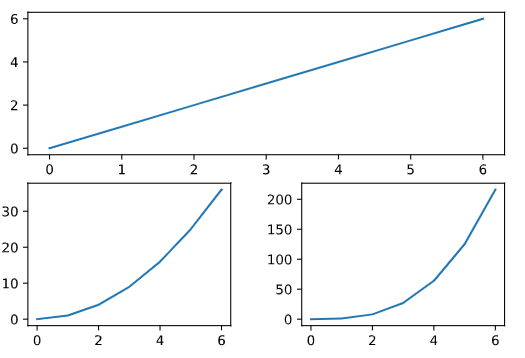
\includegraphics[scale=.55]{subadj}
	\end{minipage} \\
	We can add a \textbf{legend} to our graph, be either passing a list of strings to the .legend( ) method or passing the keywords label=`` " to the .plot method and then calling plt.legend( ) afterwards with no parameters.
	\begin{lstlisting}[language=Python]
	months = range(12)
	hyrule = [63, 65, 68, 70, 72, 72, 73, 74, 71, 70, 68, 64]
	kakariko = [52, 52, 53, 68, 73, 74, 74, 76, 71, 62, 58, 54]
	
	plt.plot(months, hyrule) # could also pass label="Hyrule"
	plt.plot(months, kakariko) # could also pass label="Kakariko"
	
	plt.legend(["Hyrule", "Kakariko"], loc=8) # default loc is 'best position'
	
	plt.show() \end{lstlisting}\vspace*{1mm}
	We can \textbf{modify tick marks} by creating an axes object and modifying the axes of that specific subplot.
	\begin{minipage}[c]{10cm}
	\begin{lstlisting}[language=Python]
	month_names = ["Jan", "Feb", "Mar", "Apr", 
	               "May", "Jun", "Jul", "Aug", 
	               "Sep","Oct", "Nov", "Dec"]
	
	months = range(12)
	conversion = [0.05, 0.08, 0.18, 0.28, 0.4, 0.66, 
	              0.74, 0.78, 0.8, 0.81, 0.85, 0.85]
	
	plt.xlabel("Months")
	plt.ylabel("Conversion")
	
	plt.plot(months, conversion)
	
	ax = plt.subplot() # create axes object
	ax.set_xticks(months) # set x ticks to months
	ax.set_xticklabels(month_names) # string labels
	ax.set_yticks([0.10, 0.25, 0.5, 0.75])
	ax.set_yticklabels(["10%", "25%", "50%", "75%"])
	
	plt.show() \end{lstlisting}\vspace*{1mm}
	\end{minipage}
	\begin{minipage}[c]{7cm}
		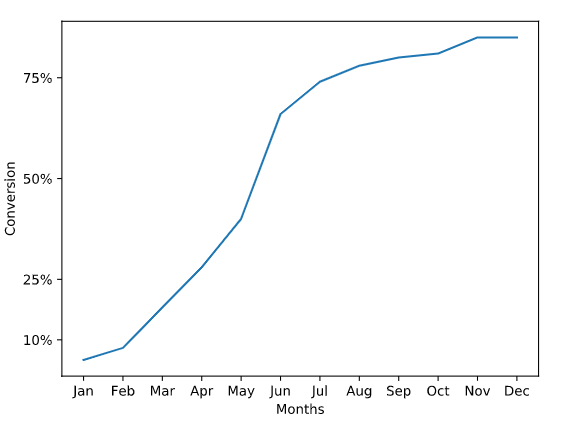
\includegraphics[scale=.52]{ticks}
	\end{minipage} \\
	We can create \textbf{figures} and save them to an output file on our system using the following commands.
	\begin{lstlisting}[language=Python]
	plt.close('all') # clear all existing plots before new one is plotted
	plt.figure(figsize=(7,3)) # creat a figure with width = 7in, height = 3in
	plt.plot(years, power_generated) # plot our data (instead of showing, save to file)
	plt.savefig('power_generated.png') # can also save as .pdf or .svg \end{lstlisting} \newpage
%%%% PAGE 19 %%%%
	\noindent LIME GRAPHING PROJECT
	\begin{lstlisting}[language=Python]
	months = ["Jan", "Feb", "Mar", "Apr", "May", "Jun", "Jul", "Aug", "Sep", "Oct", 
	          "Nov", "Dec"]
	
	visits_per_month = [9695, 7909, 10831, 12942, 12495, 16794, 14161, 12762, 
	                    12777, 12439, 10309, 8724]
	
	# numbers of limes of different species sold each month
	key_limes_per_month = [92.0, 109.0, 124.0, 70.0, 101.0, 79.0, 106.0, 101.0, 
	                       103.0, 90.0, 102.0, 106.0]
	persian_limes_per_month = [67.0, 51.0, 57.0, 54.0, 83.0, 90.0, 52.0, 63.0, 
	                           51.0, 44.0, 64.0, 78.0]
	blood_limes_per_month = [75.0, 75.0, 76.0, 71.0, 74.0, 77.0, 69.0, 80.0, 
	                         63.0, 69.0, 73.0, 82.0]
	
	plt.figure(figsize=(12,8)) # create new figure
	ax1 = plt.subplot(1,2,1) # axes object for left plot
	x_values = range(len(months))
	plt.plot(x_values, visits_per_month, marker='o')
	plt.xlabel("Months")
	plt.ylabel("Number of Visits")
	ax1.set_xticks(x_values)
	ax1.set_xticklabels(months)
	plt.title("Number of Visits per Month")
	
	ax2 = plt.subplot(1,2,2) # axes object for right plot
	plt.plot(x_values, key_limes_per_month, color='green', label='Key Limes')
	plt.plot(x_values, persian_limes_per_month, color='orange', label='Persian Limes')
	plt.plot(x_values, blood_limes_per_month, color='red', label='Blood Limes')
	plt.legend()
	ax2.set_xticks(x_values)
	ax2.set_xticklabels(months)
	plt.title("Lime Sales by Type per Month")
	
	plt.subplots_adjust(wspace=0.3)
	plt.savefig("LimeGraphComparison.png")
	plt.show() \end{lstlisting}\vspace*{1mm}
	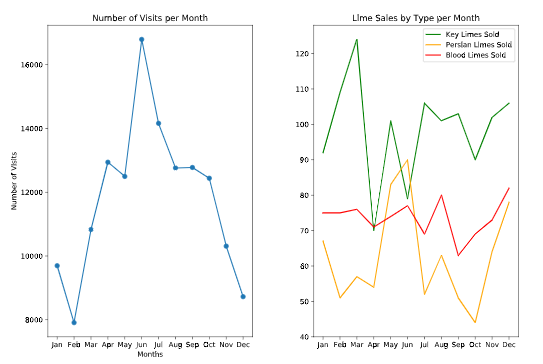
\includegraphics[scale=.95]{lime} \newpage
%%%% PAGE 20 %%%%
	\subsection{Different Plot Types \& Error}
	We can create \textbf{simple bar charts} to compare multiple categories of data with the plt.bar( ) function.\\
	\hspace*{3mm} - Note: We want our x to have the same number of elements as y, often we use range(len(y\_value))
	\begin{minipage}[c]{9cm}
	\begin{lstlisting}[language=Python]
	drinks = ["cappuccino", "latte", "chai", 
	"americano", "mocha", "espresso"]
	sales =  [91, 76, 56, 66, 52, 27]
	# create bar graph
	plt.bar(range(len(drinks)), sales) 
	# create axes object
	ax = plt.subplot()
	ax.set_xticks(range(len(drinks)))
	# label each x to corresponding drinks
	ax.set_xticklabels(drinks, rotation=20)	
	plt.show() \end{lstlisting}\vspace*{1mm}
	\end{minipage}
	\begin{minipage}[c]{8cm}
	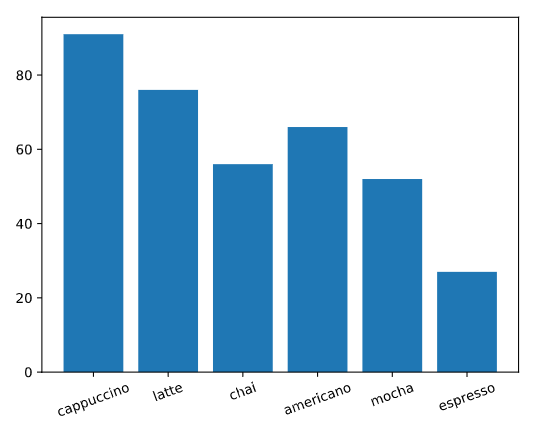
\includegraphics[scale=.5]{barchart}
	\end{minipage} \vspace*{1mm} \\
	We can use \textbf{side-by-side bar charts} to compare two sets of data with the same types of axis values. We must generate the x-axis values using list comprehension (same formula every time). \\
	\begin{minipage}[c]{9.2cm}
	\begin{lstlisting}[language=Python]
	drinks = ["cappuccino", "latte", "chai", 
	          "americano", "mocha", "espresso"]
	sales1 =  [91, 76, 56, 66, 52, 27]
	sales2 = [65, 82, 36, 68, 38, 40]
		
	n = 1  # Current dataset number
	t = 2 # Number of datasets
	d = 6 # Number of sets of bars
	w = 0.8 # Width of each bar
	store1_x = [t*element + w*n for element in 
	            range(d)]
		
	n=2 # 2nd dataset number (use prev. t,d,w)
	store2_x = [t*element + w*n for element in 
	            range(d)]
	
	plt.bar(store1_x, sales1) #plot first bar
	plt.bar(store2_x, sales2) # plot 2nd bar
	plt.show() # display graph \end{lstlisting}\vspace*{1mm}
	\end{minipage}
	\begin{minipage}[c]{8cm}
		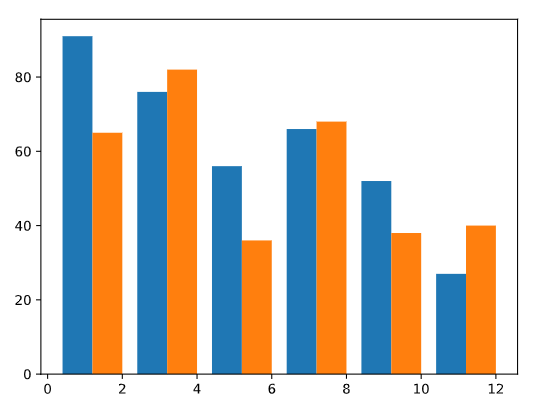
\includegraphics[scale=.57]{sidebyside}
	\end{minipage} \vspace*{1mm} \\
	We can use \textbf{stacked bar charts} to compare two data sets while preserving the total between them. We do this by plotting the first graph, then passing the keyword `bottom=' for the 2nd graph to be on top. \href{https://matplotlib.org/3.1.1/gallery/lines_bars_and_markers/bar_stacked.html}{Click here} for visual of graph style.
	\begin{lstlisting}[language=Python]
	# use datasets from above: drinks, sales1, sales2 
	
	plt.bar(range(len(drinks)), sales1, label='Location 1')
	plt.bar(range(len(drinks)), sales2, bottom=sales1, label='Location 2')
	plt.legend()
	plt.show() \end{lstlisting}\vspace*{1mm}
	We can visually represent uncertainty in our graph through using \textbf{error bars}, by passing the keywords `yerr' and `capsize' to the plt.bar( ) function. Note that you can change the error for each y-value by passing a list to yerr. (Click above link in stacked bar chart section to see example of yerr).
	\begin{lstlisting}[language=Python]
	drinks = ["cappuccino", "latte", "chai", "americano", "mocha", "espresso"]
	ounces_of_milk = [6, 9, 4, 0, 9, 0]
	error = [0.6, 0.9, 0.4, 0, 0.9, 0]
	
	plt.bar(range(len(drinks)), ounces_of_milk, yerr=error, capsize=5)
	plt.show() \end{lstlisting} \newpage
%%%% PAGE 21 %%%%
	\noindent Just like in bar charts, we can represent \textbf{error in line graphs} by using the .fill\_between( ) method and passing x-values, lower y bounds, upper y bounds, and alpha. We also must use list comprehension to calculate the upper/lower y bounds from the original y-values. (note: alpha changes error transparency).\\
	\begin{minipage}[c]{9.2cm}
	\begin{lstlisting}[language=Python]
	months = range(12)
	month_names = ["Jan", "Feb", "Mar", "Apr", 
	               "May", "Jun", "Jul", "Aug", 
	               "Sep", "Oct", "Nov", "Dec"]
	revenue = [16000, 14000, 17500, 19500, 
	           21500, 21500, 22000, 23000, 
	           20000, 19500, 18000, 16500]
	
	y_lower = [0.9*i for i in revenue]
	y_upper = [1.1*i for i in revenue]
	
	ax = plt.subplot()
	plt.fill_between(months, y_lower, y_upper, 
	                 alpha=0.2)
	plt.plot(months, revenue, marker=".")
	ax.set_xticks(months)
	ax.set_xticklabels(month_names)
	plt.show() \end{lstlisting}\vspace*{1mm}
	\end{minipage}
	\begin{minipage}[c]{8cm}
		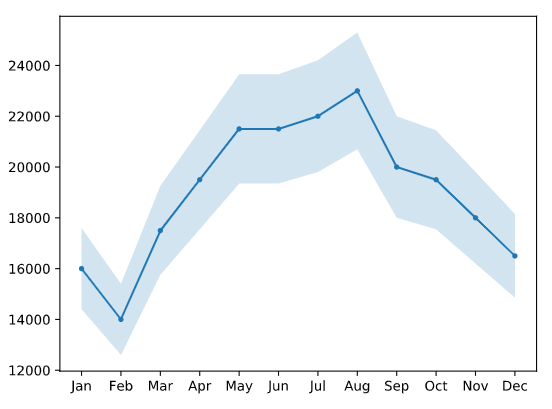
\includegraphics[scale=.57]{lineerr}
	\end{minipage} \vspace*{1mm} \\
	We can use \textbf{pie charts} to display elements of a data set as proportions of a whole by using plt.pie( ). Note that it will be tilted and we don't want this, so we must past plt.axis(``equal'') to flatten. Labeling a pie chart can be done in two different ways: \\ 
	\hspace*{3mm} - Use plt.legend( ) to create a color coded legend for each slice \\
	\hspace*{3mm} - Pass the keyword \textit{labels=` '} to plt.pie( ) to add labels on each slice \\
	We can also add the percent to the pie chart by passing the keyword autopct=` ' to the plt.pie( ) function
	\begin{lstlisting}[language=Python]
	payment_method_names = ["Card Swipe", "Cash", "Apple Pay", "Other"]
	payment_method_freqs = [270, 77, 32, 11]
	
	plt.pie(payment_method_freqs, autopct='%0.1f%%') # percent to 1 decimal place with % sign
	plt.axis('equal') # flatten our pie chart
	plt.legend(payment_method_names) # create color coded legend for graph
	plt.show() \end{lstlisting}\vspace*{1mm}
	We can create \textbf{histograms} to find a more intuitive sense for a dataset and see how many values fall in between a certain range. We do this by calling plt.hist( ). Note that we can also compare two different distribution by plotting multiple histograms, but we need to know a few keywords for this: \\
	\hspace*{3mm} - \textit{bins=} changes the number of bins to divide the data into (default is 10) \\
	\hspace*{3mm} - \textit{range=( )} to change the x-axis display value range \\
	\hspace*{3mm} - \textit{alpha=} to change the transparency of our graphs (lets us see overlap of 2 histograms) \\
	\hspace*{3mm} - \textit{histtype=`step'} will only draw the outline of our graphs (good for viewing overlap) \\
	\hspace*{3mm} - \textit{normed=True} will normalize the data so total shaded area = 1 (good for different sized data sets)
	\begin{minipage}[c]{9cm}
	\begin{lstlisting}[language=Python]
	# plot the first histogram (blue)
	plt.hist(sales_times1, bins=20, alpha=0.4, 
	         normed=True)
	         
	# plot the second histogram (orange)
	plt.hist(sales_times2, bins=20, alpha=0.4, 
	         normed=True)
	         
	plt.show() # overlap is brown \end{lstlisting}\vspace*{1mm}
	\end{minipage}
	\begin{minipage}[c]{9cm}
	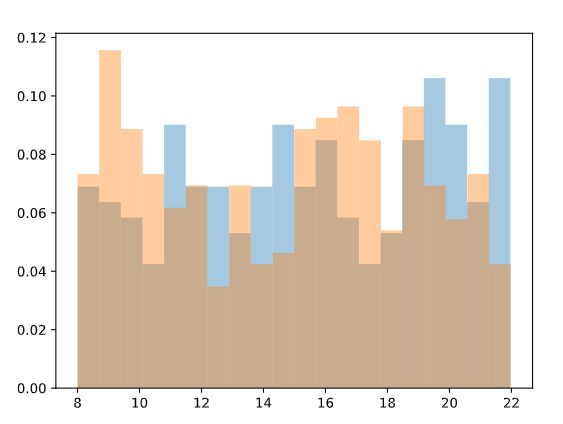
\includegraphics[scale=.48]{multhist}
	\end{minipage} \newpage
%%%% PAGE 22 %%%%
	\subsection{Selecting the Correct Visualization}
	The three steps of the data visualization process are \textit{preparing, visualizing, and styling}. We often wonder which chart to use (the visualization stage), so we can use this diagram to help us select a chart based on the data we are using and the question we are focusing on: \\~\\
	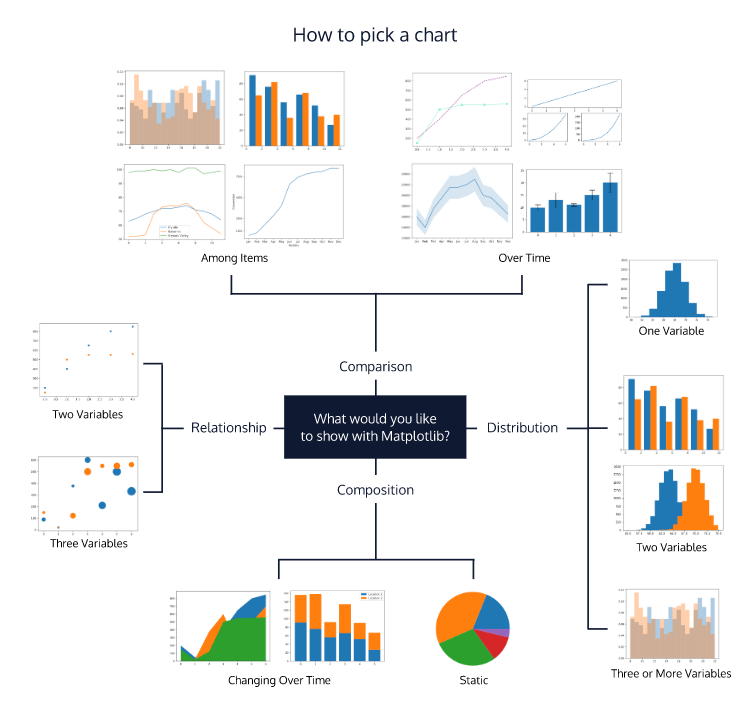
\includegraphics[scale=.8]{visdiag} \\
	\textbf{Composition Charts} - Used when asking ``what are the parts of some whole" or ``what is the data made of". Data pertaining to proportions or percentages as a whole are a good fit. \vspace*{2mm} \\
	\textbf{Distribution Charts} - Data in large quantities work well (see patterns, re-occurrences, clustering). Data that we want to see its ``distribution'' of is a good fit (such as seeing a normal dist. in statistics). \vspace*{2mm} \\
	\textbf{Relationship Charts} - Used when asking ``how do variables relate to each other". Data with two or more variables area good fit (used to see correlation between them). \vspace*{2mm} \\
	\textbf{Comparison Charts} - Used when asking ``how do variables compare to each other". Data must have multiple variables and are being used to compare against one another. \\~\\
	\textbf{Resources}: \\
	1) \href{https://s3.amazonaws.com/codecademy-content/courses/matplotlib/data_vis_matplotlib_cheatsheet_v1_revisons.pdf}{Matplotlib Cheat Sheet} from Codecademy. \\
	2) \href{https://matplotlib.org/tutorials/index.html}{Tutorials from Matplotlib website}. \\
	3) See `Constellation` project in Python folder for \underline{scatter plot} and \underline{3d rotations} in Matplotlib. \newpage
%%%% PAGE 23 %%%%
	\subsection{Introduction to Seaborn}
	Seaborn is a Python data visualization library that provides simple code to create elegant visualizations for statistical exploration and insight. Seaborn is based on Matplotlib, but improves on Matplotlib in several ways: \\	
	\hspace*{3mm} - Seaborn provides a more visually appealing plotting style and concise syntax. \\
	\hspace*{3mm} - Seaborn natively understands Pandas DataFrames, making it easier to plot data directly from CSVs. \\
	\hspace*{3mm} - Seaborn can easily summarize Pandas DataFrames with many rows of data into aggregated charts. \vspace*{2mm}\\
	Assume the following imports are all done in the examples:
	\begin{lstlisting}[language=Python]
	import pandas as pd
	from matplotlib import pyplot as plt
	import seaborn as sns
	import numpy at np \end{lstlisting}\vspace*{1mm}
	Seaborn has a much simpler way to create \textbf{bar charts} compared to Matplotlib, and we can do so with the function sns.barplot( ) and the following three keywords: \\
	\hspace*{3mm} - \textit{data=} is a Pandas DataFrame that contains the data. \\
	\hspace*{3mm} - \textit{x=} is a string that tells Seaborn which column in the DataFrame contains x-labels. \\
	\hspace*{3mm} - \textit{y=} is a string that tells Seaborn which column in the DataFrame contains y-values. \\ 
	Note: By default, Seaborn will aggregate and plot the mean of each category. 
	\begin{lstlisting}[language=Python]
	df = pd.read_csv('results.csv') # contains columns 'Gender' and 'Mean Satisfaction'
	sns.barplot(x='Gender', y='Mean Satisfaction', data= df)
	plt.show()\end{lstlisting}\vspace*{1mm}
	Seaborn can also calculate \textbf{aggregate statistics} (a single number used to describe a set of data) for large datasets. We can use NumPy to calculate these aggregates from our DataFrames. 
	\begin{lstlisting}[language=Python]
	gradebook = pd.read_csv("gradebook.csv")
	
	assignment1 = gradebook[gradebook.assignment_name == 'Assignment 1']
	asn1_median = np.median(assignment1.grade)	
	
	# Seaborn will agregate grade by assignment_name and plot average grade for both 
	# assignment 1 and assignment 2
	sns.barplot(data=gradebook, x='assignment_name', y='grade')
	plt.show()\end{lstlisting}\vspace*{1mm}
	By default, the barplot( ) function will place \textbf{error bars} (the range of values that might be expected for that bar) on all of our bars in the graph. By default, Seaborn uses a \textit{bootstrapped confidence interval} at a 95\% confidence level (but we can change the error types of these bars using the \textit{ci=} keyword). 
	\begin{lstlisting}[language=Python]
	gradebook = pd.read_csv("gradebook.csv")
	
	# change error bars to one standard deviation instead of 95% confidence intervals
	sns.barplot(data=gradebook, x="name", y="grade", ci='sd')\end{lstlisting}\vspace*{1mm}
	We can \textbf{calculate different aggregates} than just the mean of our data (Seaborn's default aggregate) by using the \textit{estimator=} keyword, which accepts any function that works on a list. Some examples: \\
	\hspace*{3mm} - np.median : use if our data has many outliers. \\
	\hspace*{3mm} - len : how many times a value appears (categorical data). 
	\begin{lstlisting}[language=Python]
	df = pd.read_csv("survey.csv")
	
	# Show how many men and women answered the survey (grouped by gender)
	sns.barplot(data=df, x='Gender', y='Response', estimator=len)
	# Show the median response value aggregated by gender
	sns.barplot(data=df, x='Gender', y='Response', estimator=np.median)\end{lstlisting}\newpage
%%%% PAGE 24 %%%%
	\noindent We can \textbf{aggregate by multiple columns} to visualize nested categorical variables. We can compare two columns at once by using the keyword \textit{hue=} to add a nested categorical variable to the plot.
	\begin{minipage}[c]{9cm}
	\begin{lstlisting}[language=Python]
	gradebook = pd.read_csv("gradebook.csv")
	
	# Visualize mean response value by gender 
	# with age range nested
	sns.barplot(data=df, x="Gender", 
	            y="Response", 
	            hue="Age Range")
	plt.show() \end{lstlisting}\vspace*{1mm}
	\end{minipage}
	\begin{minipage}[c]{10cm}
		\hspace*{5mm} 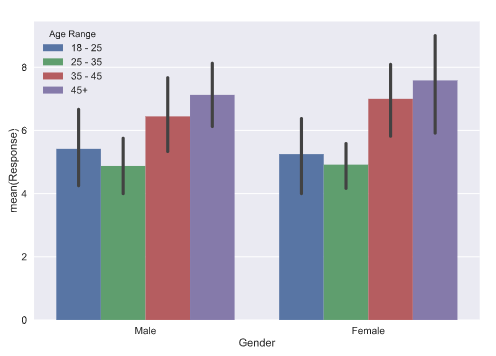
\includegraphics[scale=.5]{seamult}
	\end{minipage} \\
	\subsubsection{Plotting Distributions}
	One of the most powerful aspects of Seaborn is its ability to visualize and compare distributions. Calculating and graphing distributions is integral to analyzing massive amounts of data. We’ll look at how Seaborn allows us to communicate important statistical information through plots. \vspace*{2mm} \\
	We can use \textbf{KDE Plots} (Kernel Density Estimator) to give us the sense of a univariate (only on varaible, `one-dimensional') as a curve. KDE plots are preferable to histograms because they smooth the datasets and allow us to generalize over the shape of our data (and aren't beholden to specific data points).
	\begin{minipage}[c]{10.3cm}
	\begin{lstlisting}[language=Python]
	# Take in the data from the CSVs as NumPy arrays:
	s1 = np.genfromtxt("dataset1.csv", delimiter=",")
	s2 = np.genfromtxt("dataset2.csv", delimiter=",")
	s3 = np.genfromtxt("dataset3.csv", delimiter=",")
	s4 = np.genfromtxt("dataset4.csv", delimiter=",")
	
	sns.set_style("darkgrid") # set style
	
	# Plot the 4 datasets
	sns.kdeplot(s1, shade=True) 
	sns.kdeplot(s2, shade=True) # bimodal (two peaks)
	sns.kdeplot(s3, shade=True) # skewed left
	sns.kdeplot(s4, shade=True) # normal-ish
	plt.legend(['set 1', 'set 2', 'set 3', 'set 4'])
	plt.show() \end{lstlisting}\vspace*{1mm}
	\end{minipage}
	\begin{minipage}[c]{10cm}
	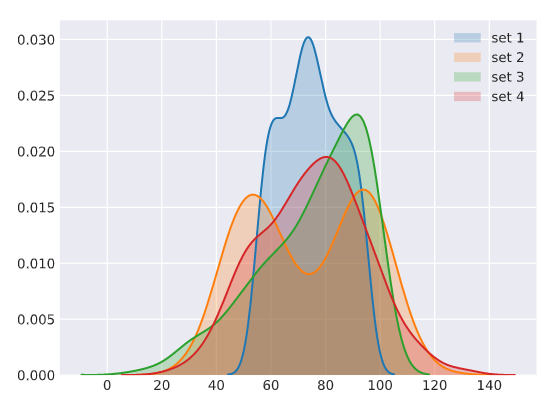
\includegraphics[scale=.48]{kde}
	\end{minipage} \\
	We can use \textbf{box plots} to show us the range of our dataset, give us an idea about where a significant portion of our data lies, and whether or not any outliers are present. We interpret a box plot as: the \textit{box} represents interquartile range, the \textit{line in the middle} of the box is the mean, the \textit{end lines} are the first and third quartiles, and the \textit{diamonds} show outliers. \\
	\hspace*{3mm} - An advantage of box plots over KDE is that it's easy to plot multiples and compare range of values. \\
	\hspace*{3mm} - Note that it shows the range of values and not the curve (distribution) of the datasets. \\
	\begin{minipage}[c]{10.3cm}
	\begin{lstlisting}[language=Python]
	n=500
	df = pd.DataFrame({ # using s1-s4 from above
	"label": ["set_one"] * n + ["set_two"] * n + 
	         ["set_three"] * n + ["set_four"] * n,
	"value": np.concatenate([s1, s2, s3, s4])
	})
	
	sns.set_style("darkgrid") # set style
	
	# Plot the 4 datasets using the dataframe
	sns.boxplot(data=df, x='label', y='value')
	plt.show()	\end{lstlisting}\vspace*{1mm}
	\end{minipage}
	\begin{minipage}[c]{10cm}
	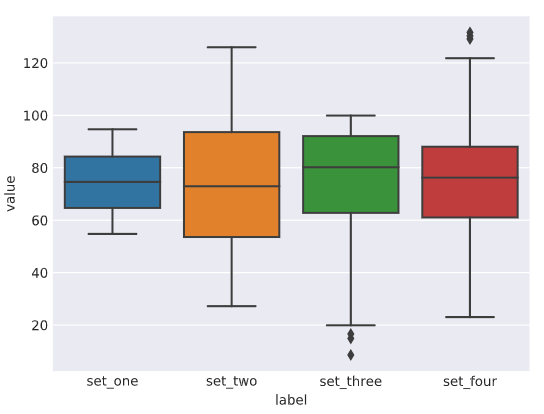
\includegraphics[scale=.48]{bpdist}
	\end{minipage} \newpage
%%%% PAGE 25 %%%%
	\noindent We can use \textbf{violin plots} to compare distributions by giving us an estimation of the dataset. It can show us the distribution (like the KDE plot) and information about the median/interquartile range (like the box plot). They are trickier to read and can be broken down to the following parts: \\
	\hspace*{3mm} - There are two \textit{KDE plots} that are symmetrical along the center line. \\
	\hspace*{3mm} - A \textit{white dot} represents the median. \\
	\hspace*{3mm} - The \textit{thick black line} in the center of each violin represents the interquartile range. \\
	\hspace*{3mm} - The \textit{lines extending from the center} are 95\% confidence intervals for our data. \\
	\begin{minipage}[c]{10.3cm}
	\begin{lstlisting}[language=Python]
	# using s1, s2, s3, and s4 from above
	# and using df from above
	
	sns.set_style("darkgrid") # set style
	
	# plot the 4 distributions using violin plot
	sns.violinplot(data=df, x='label', y='value')
	plt.show()
	# notice we see the same distributions from KDE
	# and same ranges from the boxplot \end{lstlisting}\vspace*{1mm}
	\end{minipage}
	\begin{minipage}[c]{10cm}
		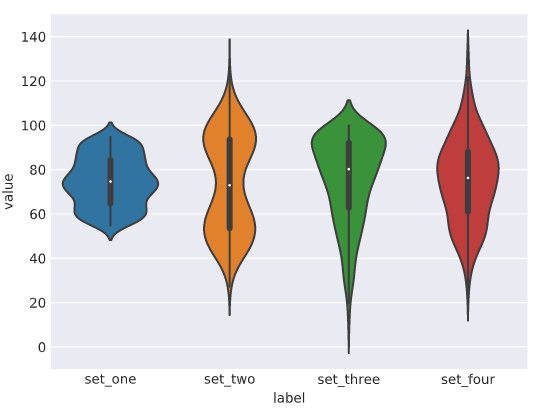
\includegraphics[scale=.48]{violin}
	\end{minipage} \\

	\subsubsection{Styling Graphs}
	Styling your graphs will influence how your audience understands what you're trying to convey. When deciding the style, ask yourself: is it part of a report, is it part of a presentation, is it stand alone with no explanation? These questions will help decide which style to chose in order to best convey your data. \\~\\
	Seaborn has five \textbf{built in themes}: darkgrid, whitegrid, dark, white, and ticks. All of which can be passed into the sns.set\_style( ) method. \vspace*{2mm} \\
	It is important to consider \textbf{background color}. The higher the contrast between you plot color palette and the figure background, the more legible the data visualization will be. \vspace*{2mm} \\
	Including a \textbf{grid} can be helpful when you want your audience to be able to draw their own conclusions about data. Research papers and reports are a good example of when you would want to include a grid.\vspace*{2mm} \\
	We can remove \textbf{spines} from plots (the four black borders that contain the graph) by using sns.despine(), which by default will remove the top/right spines (can pass \textit{left=True, bottom=True} to remove all spines).\vspace*{2mm} \\
	We can \textbf{customize plots for presentation} by using sns.set\_context( ) and passing these keywords: \\
	\hspace*{3mm} - the first parameter adjusts the scale of the plot: `paper', `notebook', `talk', `poster'. \\
	\hspace*{3mm} - \textit{font\_scale=} will change the size of the text. \\
	\hspace*{3mm} - \textit{rc=} will let us change any value in a dictionary (run sns.plotting\_context() to see which values can 
	\hspace*{5.5mm} be changed). \vspace*{2mm} \\
	We can change \textbf{palette color} with two different functions, sns.color\_palette( ) and sns.set\_pallete( ). \\
	\hspace*{3mm} - sns.color\_palette( ) can be saved to a variable, then passed in sns.palplot( ) to see an array of colors. \\
	\hspace*{3mm} - sns.set\_pallete( ) is passed the name of the pallete you want to use for the plot. \vspace*{2mm} \\
	Note: you can also use \href{https://colorbrewer2.org/#type=sequential&scheme=BuGn&n=3}{Color Brewer Palettes} instead of the default Seaborn colors by passing the name and number of colors needed.
	\begin{lstlisting}[language=Python]
	palette = sns.color_palette("bright") # to visualize the colors in a pallete
	sns.palplot(palette) 
	
	sns.set_palette("Paired") # to set the pallete for the plot
	
	sns.set_palette("Set3", 10) # color brewer pallete with 10 different shades	\end{lstlisting} \newpage
%%%% PAGE 26 %%%%
	\subsection{Data Visualization Cumulative Projects}
	
	
	
	 
\end{spacing}
\end{document}




